\documentclass[11pt]{article}
\usepackage[margin=1in]{geometry}
\usepackage{tikz}
\usetikzlibrary{arrows.meta,positioning}

\title{Investment Platform Vision (v1)}
\date{}

\begin{document}
\maketitle

\section*{Future Vision Summary}
Build an autonomous research and tracking investment platform that:
\begin{itemize}
  \item researches market opportunities continuously,
  \item tracks portfolio decisions and outcomes,
  \item adapts strategies from updated vision documents.
\end{itemize}

\section*{System View}
\begin{center}
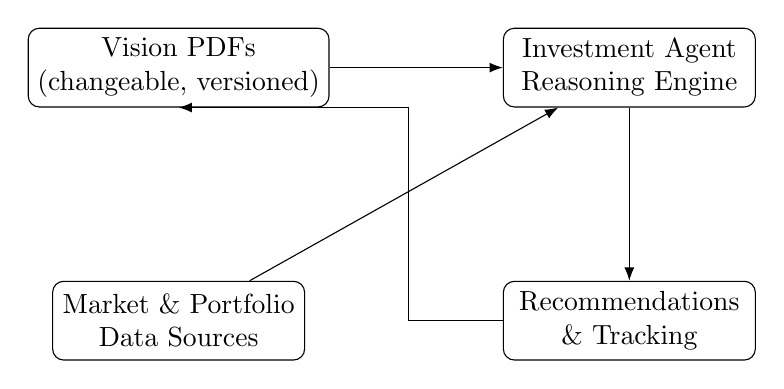
\begin{tikzpicture}[
  node distance=2.2cm,
  block/.style={draw, rounded corners, align=center, minimum width=3.2cm, minimum height=1cm},
  >={Latex}
]
\node[block] (vision) {Vision PDFs\\(changeable, versioned)};
\node[block, right=of vision] (engine) {Investment Agent\\Reasoning Engine};
\node[block, below=of vision] (data) {Market \& Portfolio\\Data Sources};
\node[block, below=of engine] (actions) {Recommendations\\\& Tracking};

\draw[->] (vision) -- (engine);
\draw[->] (data) -- (engine);
\draw[->] (engine) -- (actions);
\draw[->] (actions.west) -- ++(-1.2,0) |- (vision.south);
\end{tikzpicture}
\end{center}

\end{document}
